% Section 7, Results.
\section{Results}
\label{sec:results}

% ---------------------------------------------------------------------------
% 7.1  Headline
% ---------------------------------------------------------------------------
\subsection{Headline}
\label{sec:results-headline}

\begin{table}[!tbp]
\centering
\caption{\textbf{Main results on SWE-bench Pro (Python-266).}
\sysname matches the pool's best single model (\fxopus) at about a fifth
of its cost per solve; 159 versus 158 is a one-task gap at $n{=}266$, a
match, not a win.  The last row is the no-router ablation, which ties
the routed system on this benchmark (\S\ref{sec:results-headline}).}
\label{tab:main-results}
% ===========================================================================
% tab-main-results.tex — main results, SWE-bench Pro Python-266.
% BODY ONLY (tabular): the table wrapper, \caption and \label live in the
% section file that includes this.
% Provenance: data/receipts/outcomes_per_task.json.
%
% "vs. mix" = percentage points above the blind-mixing line, i.e. the linear
%   interpolation between the two solo endpoints, \fxkimi ($0.106138/task,
%   56.0150%) -> \fxopus ($0.756586/task, 59.3985%) in ($/task, solve-rate)
%   space, evaluated at the row's own $/task; row rates use the exact
%   fraction 159/266, not the rounded 59.77%.
% Bolding: best value per column; genuine ties are bolded on both rows.
%   Wording rule: "matches", never "beats" — 159 vs 158 is one task at n=266.
% Layout: wide table. House rule is a smaller font plus tighter \tabcolsep
%   kept local to this tabular, never \resizebox. The first column is a
%   fixed-width paragraph column so the two long system labels wrap instead
%   of pushing the tabular past the text column.
% ===========================================================================
\begingroup\footnotesize\setlength{\tabcolsep}{2pt}%
\begin{tabular}{@{}p{1.20in}rrrrr@{}}
\toprule
System & Solves/266 & Rate & \$/task & \$/solve & vs.\ mix \\
\midrule
\raggedright\sysname (router, $\theta{=}0.30$)
  & \textbf{159} & \textbf{59.77\%} & \$0.137 & \$0.230 & $+3.60$ \\
\midrule
\fxopus solo  & 158 & 59.40\% & \$0.757 & \$1.274 & --- \\
\fxkimi solo  & 149 & 56.02\% & \textbf{\$0.106} & \textbf{\$0.190} & --- \\
\fxgpt solo   & 139 & 52.26\% & \$0.570 & \$1.091 & --- \\
\midrule
\raggedright No-router ablation (\fxkimi $+$ handoff)
  & \textbf{159} & \textbf{59.77\%} & \$0.136 & \$0.227 & $+3.60$ \\
\bottomrule
\multicolumn{6}{@{}p{0.97\linewidth}@{}}{\footnotesize Solves are out of
$n{=}266$, top to bottom: 159, 158, 149, 139, 159. The \sysname row and the
ablation row share one all-in cost convention: fixer API spend plus the
\modelname searcher's GPU bill plus verify-then-strip sandbox infrastructure,
amortized over 266 tasks. Solo rows are fixer API spend only. ``vs.\ mix'' is
percentage points above the \fxkimi--\fxopus blind-mixing line at the row's
own \$/task.}
\end{tabular}%
\endgroup

\end{table}

Table~\ref{tab:main-results} summarizes the primary evaluation.
\sysname solves 159 of 266 tasks (59.77\%) at a total cost per solve of
\$0.230.  The pool's best single model, \fxopus run solo, solves 158 of
266 (59.40\%) at \$1.274 per solve.  \sysname matches this ceiling at
about a fifth of the cost per solve.  The one-task gap between 159 and
158 at $n{=}266$ is not a meaningful difference; it is a match.

The no-router ablation sends every task to \fxkimi with the handoff and
no routing decision at all, also solving 159 of 266 at \$0.227 per
solve.  The calibrated router concentrates 263 of 266 tasks on the
cheapest fixer and adds no solves over this ablation; its three
diversions to \fxflash~\citep{gemini3flash} cost \$0.003 per solve,
insurance rather than accuracy.  On this benchmark, then, the handoff
carries the result and routing collapses to cost allocation.  Whether
blanket assignment to one cheap fixer reaches parity is a property of
this pool and benchmark, not a general rule: in deployment that answer
is not known in advance, and the router is the component that predicts
it, from free public data, before any spend.  The ablation is ex-ante
specifiable too, but only hindsight shows it reaches parity; the router
turns that gamble into a calibrated decision.  Both
system rows sit above the blind-mixing line defined in
\S\ref{sec:setup} by $+$3.60 percentage points at their respective cost
points (visible in Figure~\ref{fig:cost-solve}).  \modelname's entire
GPU bill for all 266 search episodes was \$1.13, under half a cent per
task.

Why were both frontier models run in full as solo baselines?  Our
calibration study and a small paid probe disagreed about which was
stronger.  On the fresh calibration tasks (\S\ref{sec:calibration}),
\fxgpt was the strongest solo fixer at 60.6\% solve rate.  A small paid
probe of 15 tasks per fixer leaned the other way: \fxopus solved two
more tasks, but $p{=}0.625$, well below the pre-declared decision bar,
while inverting the calibration prior.  Both were therefore run in full.
The complete paired comparison resolved the question: \fxopus beats
\fxgpt by $+$7.14 percentage points on the same 266 tasks, with 44
tasks solved only by \fxopus versus 25 solved only by \fxgpt (exact
McNemar test~\citep{mcnemar}, $p{=}0.029$).

One further observation from the solo baselines deserves note.
\fxkimi solo resolves 149 of 266 tasks (56.02\%) at \$0.106 per task,
dominating \fxgpt solo (139/266, 52.26\%, \$0.570 per task) on both
axes, gaining $+$3.76 percentage points of accuracy at roughly one fifth
of the per-task cost.

% ---------------------------------------------------------------------------
% 7.2  Component Analysis
% ---------------------------------------------------------------------------
\subsection{Component Analysis}
\label{sec:results-components}

\paragraph{Localization quality.}

\begin{table}[!tbp]
\centering
\caption{\textbf{\modelname's file localization on SWE-bench Pro
(Python-266).}  Per-task mean recall and precision against the gold
patch's file set.  Spontaneous and forced handoffs are reported
separately.  All numbers are from a single sampled draw at
temperature~$0.9$ (no majority vote).}
\label{tab:localization}
% ===========================================================================
% tab-localization.tex — \modelname file localization quality on Pro-266.
% BODY ONLY (tabular). Wrapper/caption/label live in the section file.
%
% PROVENANCE — every cell.
%   Source: internal records.
%     overall row (n=266)      = overall: mean recall 0.566,
%                                mean precision 0.821, all-gold-hit 24.8%
%     spontaneous row (n=206)  = spontaneous vs forced,
%                                spontaneous column: 0.586 / 0.833 / 28.2%
%     forced row (n=60)        = forced column: 0.499 / 0.780 / 13.3%
%   Method (single sampled draw, temp 0.9, no majority vote; gold = b-side
%   `diff --git` paths of `gold_patch`) = the source's method and caveats.
%
%   RULE APPLIED: the per-repo breakdown (ansible / openlibrary /
%   qutebrowser) is APPENDIX-ONLY and is
%   deliberately omitted here.
%   Spontaneous and forced are NEVER pooled in the row-level breakdown; the
%   overall row pools them only for the single top-line number, per the
%   source's own rule.
% ===========================================================================
\begin{tabular}{@{}lrrr@{}}
\toprule
Handoff type & Recall & Precision & All-gold \\
\midrule
Overall ($n{=}266$)      & 0.566 & 0.821 & 24.8\% \\
\midrule
Spontaneous ($n{=}206$)  & \textbf{0.586} & \textbf{0.833} & \textbf{28.2\%} \\
Forced ($n{=}60$)        & 0.499 & 0.780 & 13.3\% \\
\bottomrule
\end{tabular}

\end{table}

Table~\ref{tab:localization} reports the quality of \modelname's file
localization.
Against a mean of 3.44 gold files per task, the searcher names a median
of 2.0 files, achieving per-task mean recall of 0.566 and precision of
0.821; in 24.8\% of tasks every gold file appears in the handoff.
Spontaneous handoffs ($n{=}206$) localize substantially better than
forced ones ($n{=}60$) across the board: recall 0.586 versus 0.499,
precision 0.833 versus 0.780, and all-gold rate 28.2\% versus 13.3\%.
This gap is unsurprising: tasks that exhaust the turn budget are
typically harder.  It underscores why the two handoff types are
never pooled when reporting component behavior (per-repository detail in Appendix~\ref{apx:localization}).

\paragraph{Verify-then-strip guard.}
Of 266 handoffs, 249 included a claimed verified reproduction of the
bug.  Replaying every claim inside the task sandbox revealed that only
50 of them (20\%) were genuine, while 174 (70\%) were demonstrably
false.  The guard stripped every false claim before any fixer saw it.
Forced handoffs overclaimed more aggressively: just 9\% of their
reproduction claims were genuine, compared with 22\% for spontaneous
handoffs.
These benchmark rates are worse than those observed during calibration
(32\% genuine, 56\% false; \S\ref{sec:calibration}), consistent with
harder tasks producing more overclaiming.
The guard neutralizes this overclaiming before any fixer sees it: 174
fixer prompts were stripped of confident misinformation that would
otherwise have been treated as ground truth (full outcome classes in
Appendix~\ref{apx:verify-strip}); we did not run a pass-through arm, so
the guard's contribution to the headline is an inference from this
claim census rather than a measurement (\S\ref{sec:limitations}).

\paragraph{Protocol findings.}
The auto-submit-at-cap mechanism rescued 24 of \fxopus's 158 solves and
33 of \fxgpt's 139.  Without it, both frontier models' solve rates would read
roughly 9--13 percentage points lower.
The 50-call cap binds often: it was reached in 36.5\% of \fxgpt
attempts, 17.3\% of \fxopus attempts, and 48\% of \fxkimi attempts.
The \$2 cost cap bound only 5 times (all \fxopus, maximum \$2.09).
The gold-control census confirmed 265 of 266 tasks
(\S\ref{sec:setup}) (full cap statistics in Appendix~\ref{apx:cap-stats}).

\paragraph{Router behaviour.}

\begin{figure}[!tbp]
\centering
% ===========================================================================
% fig-gate-probability.tex — distribution of the router's gate probability for
% the cheapest fixer, under three feature spaces.
% BODY ONLY (tikzpicture). Wrapper/caption/label live in the section file.
% Requires % ===========================================================================
% fig-style.tex — shared colour / marker scheme for EVERY main-paper figure.
% \input this ONCE from the preamble of main.tex (after tikz + pgfplots).
%
% House rule: the palette is defined here and nowhere else. Each series also
% gets a distinct marker AND line style so the figures survive grayscale
% printing.
%
%   \sysname / deployed .. cSys   (blue!70!black)    mark *
%   opus / claude ........ cOpus  (red!70!black)     mark square*
%   gpt .................. cGpt   (teal!70!black)    mark triangle*
%   kimi ................. cKimi  (violet!70!black)  mark diamond*
%   flash ................ cFlash (orange!70!black)  mark pentagon*
%   greedy / baseline .... cBase  (gray)             mark o
% ===========================================================================
% The pipeline diagram needs the calc library for coordinate arithmetic; the
% rest of the libraries are already loaded in main.tex's preamble.
\usetikzlibrary{calc}
% Hatching, so bar charts stay readable in grayscale.
\usetikzlibrary{patterns}

\colorlet{cSys}{blue!70!black}
\colorlet{cOpus}{red!70!black}
\colorlet{cGpt}{teal!70!black}
\colorlet{cKimi}{violet!70!black}
\colorlet{cFlash}{orange!70!black}
\colorlet{cBase}{gray}

% Common axis furniture: footnotesize ticks/legend, small titles, framed
% legend in gray!50, light horizontal grid.
\pgfplotsset{
  paperaxis/.style={
    width=0.80\linewidth,
    height=5.2cm,
    tick label style={font=\footnotesize},
    label style={font=\footnotesize},
    title style={font=\small},
    legend style={font=\footnotesize, draw=gray!50, fill=white,
                  fill opacity=0.9, text opacity=1, rounded corners=1pt},
    every axis plot/.append style={line width=0.7pt},
    grid style={gray!25, line width=0.3pt},
    axis line style={gray!60},
    tick style={gray!60},
  },
  papermark/.style={mark size=2.6pt},
}
 in the preamble.
% Provenance: data/receipts/routing_scenarios.json — per-task probabilities
% read from the probability_vectors map for the cheapest fixer (first entry of
% cheap_order), three fields per task: p_state (hidden-state head, cSys solid),
% p_text (task-text head, cBase dashed) and p_blend (their uniform average, the
% routing head the gate thresholds, cOpus dotted). n = 266.
%
% Binning: 19 equal bins of width 0.05, left edges 0.05 ... 0.95, half-open
% [lo, hi) with the last bin closed; each series sums to 266. Plotted as
% const-plot outlines, coordinates (left edge, count), opened with (0.05,0)
% and closed with (1.00,0). theta = 0.30 is the only threshold drawn.
% ===========================================================================
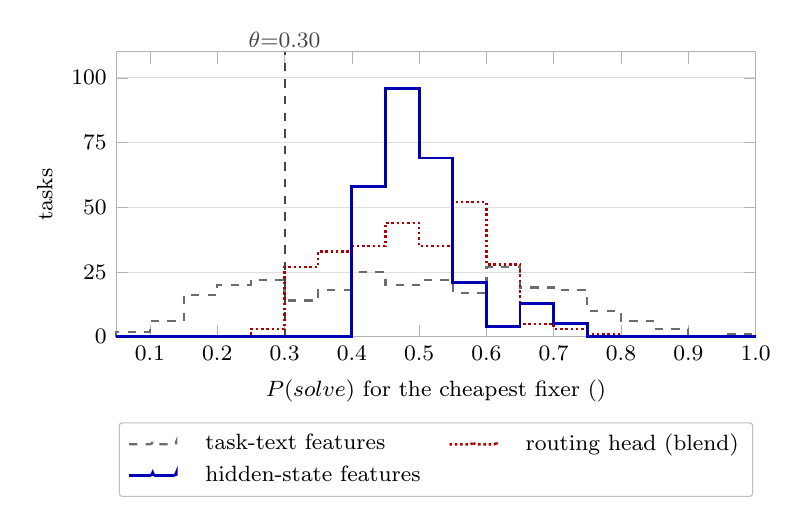
\begin{tikzpicture}
\begin{axis}[
  paperaxis,
  width=0.80\linewidth,
  height=5.2cm,
  xmin=0.05, xmax=1.00,
  ymin=0, ymax=110,
  xtick={0.1,0.2,0.3,0.4,0.5,0.6,0.7,0.8,0.9,1.0},
  xticklabel style={/pgf/number format/fixed,
                    /pgf/number format/fixed zerofill,
                    /pgf/number format/precision=1},
  ytick={0,25,50,75,100},
  xlabel={$P(\text{solve})$ for the cheapest fixer (\fxkimi)},
  ylabel={tasks},
  ymajorgrids=true,
  clip=false,   % lets the \theta tag sit just above the top frame
  legend style={at={(0.5,-0.30)}, anchor=north, legend columns=2,
                column sep=8pt},
  legend cell align=left,
]

% ---- deployed threshold, the ONLY threshold drawn ----------------------
\addplot[gray!55!black, line width=0.7pt, dashed, forget plot]
  coordinates {(0.30,0) (0.30,110)};
\node[font=\footnotesize, text=gray!55!black, anchor=south, inner sep=1.5pt]
  at (axis cs:0.30,110) {$\theta{=}0.30$};

% ---- task-text features (widest, drawn first so it sits behind) --------
\addplot[const plot, cBase!85!black, line width=0.8pt, dashed]
  coordinates {(0.05,0)
    (0.05,2) (0.10,6) (0.15,16) (0.20,20) (0.25,22) (0.30,14)
    (0.35,18) (0.40,25) (0.45,20) (0.50,22) (0.55,17) (0.60,27)
    (0.65,19) (0.70,18) (0.75,10) (0.80,6) (0.85,3) (0.90,0)
    (0.95,1) (1.00,0)};
\addlegendentry{task-text features}

% ---- routing head (uniform average of the two feature heads) -----------
\addplot[const plot, cOpus, line width=0.9pt, densely dotted]
  coordinates {(0.05,0)
    (0.05,0) (0.10,0) (0.15,0) (0.20,0) (0.25,3) (0.30,27)
    (0.35,33) (0.40,35) (0.45,44) (0.50,35) (0.55,52) (0.60,28)
    (0.65,5) (0.70,3) (0.75,1) (0.80,0) (0.85,0) (0.90,0)
    (0.95,0) (1.00,0)};
\addlegendentry{routing head (blend)}

% ---- hidden-state features (the concentrated one, drawn last, on top) --
\addplot[const plot, cSys, line width=1.0pt]
  coordinates {(0.05,0)
    (0.05,0) (0.10,0) (0.15,0) (0.20,0) (0.25,0) (0.30,0)
    (0.35,0) (0.40,58) (0.45,96) (0.50,69) (0.55,21) (0.60,4)
    (0.65,13) (0.70,5) (0.75,0) (0.80,0) (0.85,0) (0.90,0)
    (0.95,0) (1.00,0)};
\addlegendentry{hidden-state features}

\end{axis}
\end{tikzpicture}

\caption{\textbf{Two feature spaces, two very different confidence
distributions at the routing gate ($\theta{=}0.30$).}  Histograms of
$P(\text{solve})$ for \fxkimi (cheapest fixer) across all $266$ tasks.
The task-text head spans nearly the full unit interval (sd~$0.20$),
while the hidden-state head concentrates tightly (sd~$0.07$, support
entirely above~$\theta$).  Their blend, the routing head, gates $263$ of
$266$ tasks to the cheapest fixer.}
\label{fig:gate-probability}
\end{figure}

The router sends 263 of 266 tasks to \fxkimi: the first fixer in
cheap-to-expensive order whose blended solve probability clears
$\theta{=}0.30$ receives the task.
Figure~\ref{fig:gate-probability} reveals how the two underlying feature
spaces distribute that probability.  The task-text head spreads wide
(sd~$0.20$, support $0.08$--$0.97$), while the hidden-state head
concentrates tightly (sd~$0.07$, support $0.40$--$0.74$) and sits
entirely above the threshold.
Because that support lies entirely above $\theta$, part of the
hidden-state head's effect at the gate is mechanical: blending shrinks
the text head's predictions toward the state head's near-constant mean,
which by itself admits more tasks to the cheapest fixer.  We did not
run a matched shrinkage control, so the feature's informational
contribution cannot be fully separated from this threshold-shifting
effect; the held-out separation gap (AUC $0.600$ versus $0.561$ for
task text at $N{=}99$, Appendix~\ref{apx:design-space}) is suggestive
rather than decisive.
The hidden state's contribution is not boosting accuracy per se but
shifting \emph{when} the cheap model is trusted, consistent with its
cost-side rather than accuracy-side value observed during
calibration~(\S\ref{sec:calibration}).

\FloatBarrier

% ---------------------------------------------------------------------------
% 7.3  Onboarding
% ---------------------------------------------------------------------------
\subsection{Onboarding a New Fixer}
\label{sec:results-onboarding}

\begin{figure}[!tbp]
\centering
% ===========================================================================
% fig-onboarding.tex — onboarding a new fixer in three steps.
% BODY ONLY (tikzpicture in a \resizebox). Wrapper/caption/label live in the
% section file; mounts as a single-column \begin{figure}[!tbp].
% Requires % ===========================================================================
% fig-style.tex — shared colour / marker scheme for EVERY main-paper figure.
% \input this ONCE from the preamble of main.tex (after tikz + pgfplots).
%
% House rule: the palette is defined here and nowhere else. Each series also
% gets a distinct marker AND line style so the figures survive grayscale
% printing.
%
%   \sysname / deployed .. cSys   (blue!70!black)    mark *
%   opus / claude ........ cOpus  (red!70!black)     mark square*
%   gpt .................. cGpt   (teal!70!black)    mark triangle*
%   kimi ................. cKimi  (violet!70!black)  mark diamond*
%   flash ................ cFlash (orange!70!black)  mark pentagon*
%   greedy / baseline .... cBase  (gray)             mark o
% ===========================================================================
% The pipeline diagram needs the calc library for coordinate arithmetic; the
% rest of the libraries are already loaded in main.tex's preamble.
\usetikzlibrary{calc}
% Hatching, so bar charts stay readable in grayscale.
\usetikzlibrary{patterns}

\colorlet{cSys}{blue!70!black}
\colorlet{cOpus}{red!70!black}
\colorlet{cGpt}{teal!70!black}
\colorlet{cKimi}{violet!70!black}
\colorlet{cFlash}{orange!70!black}
\colorlet{cBase}{gray}

% Common axis furniture: footnotesize ticks/legend, small titles, framed
% legend in gray!50, light horizontal grid.
\pgfplotsset{
  paperaxis/.style={
    width=0.80\linewidth,
    height=5.2cm,
    tick label style={font=\footnotesize},
    label style={font=\footnotesize},
    title style={font=\small},
    legend style={font=\footnotesize, draw=gray!50, fill=white,
                  fill opacity=0.9, text opacity=1, rounded corners=1pt},
    every axis plot/.append style={line width=0.7pt},
    grid style={gray!25, line width=0.3pt},
    axis line style={gray!60},
    tick style={gray!60},
  },
  papermark/.style={mark size=2.6pt},
}
 in the preamble.
%
% PROVENANCE
%   Schematic, illustrative only, no measured quantities. The only quantity
%   drawn is the documented spec constant 25--50 public per-task outcomes,
%   which is stated with its source in \S\ref{sec:results-onboarding} and
%   Table~\ref{tab:router-recipe}; nothing else in the figure is a number,
%   and no model or benchmark is named.
%
%   Glyph continuity: the r\'esum\'e card in step 2 and the fixer chips plus
%   dashed open slot in step 3 repeat the glyphs used in fig-pipeline.tex
%   (the r\'esum\'e shelf beneath the router, and the fixer-pool chips), so a
%   reader recognises the same objects across the two figures.
%
%   Colour contract (fig-style.tex): cSys tints only what onboarding adds
%   (the new r\'esum\'e, the new chip); everything already in the system is
%   neutral gray, which is also the point of the frozen strip along the
%   bottom. Fills differ in lightness, so the figure survives grayscale.
% ===========================================================================
\resizebox{\linewidth}{!}{%
\begin{tikzpicture}[
  x=1cm, y=1cm,
  panel/.style={rounded corners=2.2pt, line width=0.7pt, draw=gray!50,
                fill=gray!3, anchor=center},
  kick/.style={font=\scriptsize\scshape, text=gray!45!black, anchor=south,
               inner sep=0pt},
  head/.style={font=\footnotesize\bfseries, text=gray!20!black,
               anchor=north, align=center, inner sep=0pt},
  micro/.style={font=\scriptsize, text=gray!42!black, anchor=north,
                align=center, inner sep=0pt},
  flow/.style={-{Stealth[length=1.9mm,width=1.4mm]}, gray!62,
               line width=0.9pt},
]

% =========================================================================
% Geometry: three 2.55cm panels, 2.85cm tall, centred on y=0, with 0.50cm
% gaps for the arrows.  Centres: 1.275 / 4.325 / 7.375; drawing width 8.65.
% =========================================================================
\def\Pw{2.55} \def\Ph{2.85}

\node[panel, minimum width=\Pw cm, minimum height=\Ph cm] (s1) at (1.275,0) {};
\node[panel, minimum width=\Pw cm, minimum height=\Ph cm] (s2) at (4.325,0) {};
\node[panel, minimum width=\Pw cm, minimum height=\Ph cm] (s3) at (7.375,0) {};

\node[kick] at (1.275,1.52) {Step 1};
\node[kick] at (4.325,1.52) {Step 2};
\node[kick] at (7.375,1.52) {Step 3};

\draw[flow] (s1) -- (s2);
\draw[flow] (s2) -- (s3);

% =========================================================================
% Shared per-panel layout: heading north-anchored at y = 1.30, glyph in the
% band y = -0.70 .. 0.70, one-line-or-two caption north-anchored at -0.80.
% =========================================================================

% ---- Step 1 — collect a short public outcome record ---------------------
\node[head, text width=2.35cm] at (1.275,1.30) {Collect outcomes};
\foreach \i/\m/\c in {0/{$\times$}/{gray!68}, 1/{$\checkmark$}/{gray!58},
                      2/{$\times$}/{gray!68}, 3/{$\checkmark$}/{gray!58}}{
  \draw[draw=gray!45, fill=white, line width=0.5pt, rounded corners=1.2pt]
    (0.400,-0.62+0.30*\i) rectangle ++(1.75,0.26);
  \node[font=\scriptsize, text=\c, inner sep=0pt]
    at (0.60,-0.49+0.30*\i) {\m};
  \draw[gray!35, line width=0.4pt]
    (0.80,-0.49+0.30*\i) -- (2.00,-0.49+0.30*\i);
}
\node[micro, text width=2.35cm] at (1.275,-0.80)
  {25--50 public\\per-task outcomes};

% ---- Step 2 — average into a résumé (glyph mirrors fig-pipeline.tex) ----
\node[head, text width=2.35cm] at (4.325,1.30) {Average into\\a r\'esum\'e};
\draw[gray!45, fill=white, line width=0.5pt, rounded corners=1.2pt]
  (3.535,-0.41) rectangle ++(1.70,0.94);
\draw[cSys!60, fill=cSys!14, line width=0.7pt, rounded corners=1.2pt]
  (3.475,-0.47) rectangle ++(1.70,0.94);
\fill[cSys!75] (3.635,0.24)  circle (1.9pt);
\fill[gray!48] (3.635,-0.02) circle (1.9pt);
\node[font=\scriptsize, text=gray!35!black, anchor=west, inner sep=0pt]
  at (3.775,0.245) {solved};
\node[font=\scriptsize, text=gray!35!black, anchor=west, inner sep=0pt]
  at (3.775,-0.015) {failed};
\draw[gray!45, line width=0.4pt] (3.615,-0.28) -- (5.035,-0.28);
\fill[cSys!45] (3.615,-0.33) rectangle (4.265,-0.23);
\node[micro, text width=2.4cm] at (4.325,-0.80)
  {two centroids\\$+$ a base rate};

% ---- Step 3 — routable at once (chips mirror fig-pipeline.tex) ----------
\node[head, text width=2.35cm] at (7.375,1.30) {Routable at once};
\foreach \i in {0,1,2}{
  \draw[draw=gray!38, fill=white, line width=0.55pt, rounded corners=1.4pt]
    (6.400,0.40-0.34*\i) rectangle ++(1.95,0.28);
  \fill[gray!48] (6.480,0.46-0.34*\i) rectangle ++(0.08,0.16);
  \node[font=\scriptsize, text=gray!45!black, anchor=west, inner sep=0pt]
    at (6.680,0.54-0.34*\i) {existing fixer};
}
% the open slot, and the new fixer landing in it
\draw[draw=gray!45, dash pattern=on 0.8mm off 0.7mm, line width=0.5pt,
      rounded corners=1.4pt] (6.380,-0.76) rectangle ++(1.95,0.28);
\draw[draw=cSys!70, fill=cSys!14, line width=0.85pt, rounded corners=1.4pt]
  (6.500,-0.67) rectangle ++(1.95,0.28);
\fill[cSys] (6.580,-0.61) rectangle ++(0.08,0.16);
\node[font=\scriptsize\bfseries, text=cSys!72!black, anchor=west,
      inner sep=0pt] at (6.780,-0.53) {new fixer};
\node[micro, text width=2.45cm] at (7.375,-0.92)
  {the router reads it};

% =========================================================================
% The frozen strip: nothing retrains
% =========================================================================
\draw[gray!45, fill=gray!6, line width=0.5pt, rounded corners=2.2pt]
  (0,-2.28) rectangle (8.65,-1.72);
\node[font=\scriptsize\itshape, text=gray!42!black] at (4.325,-2.00)
  {searcher, embedder, scorer: all frozen, nothing retrains};

\end{tikzpicture}}

\caption{\textbf{Onboarding a fixer costs a r\'esum\'e, not a training
run.} A short public outcome record averages into two centroids and a base
rate, and the router reads that r\'esum\'e at inference time. No component
is retrained.}
\label{fig:onboarding}
\end{figure}

Adding a new fixer requires no retraining.
A fixer's \emph{r\'esum\'e} consists of two averaged embeddings (one
over its solved tasks, one over its failed tasks) plus a base solve
rate, all buildable from 25--50 public per-task outcomes
(Table~\ref{tab:router-recipe}).
The embedder is frozen infrastructure and \modelname never retrains; the
router simply reads each new r\'esum\'e at inference time
(Figure~\ref{fig:onboarding}).
This design keeps the pool extensible: a fixer released tomorrow can be
routed to as soon as a short public-benchmark run produces its outcome
record.
Appendix~\ref{apx:bench-fresh} bounds what such public outcomes can
carry: on our fresh calibration tasks every fixer's public rate drops
and the public ordering does not survive.
A r\'esum\'e built from public outcomes is therefore a cold-start
device, adequate for admitting a new fixer to the pool but not for
fine-grained ranking, and the thresholds used in this paper were
calibrated on freshly measured labels for exactly this reason.
